\documentclass[14pt, a4paper]{article}
\usepackage{minitoc}
\usepackage[left=3.00cm, right=2.5cm, top=2.00cm, bottom=2.00cm]{geometry}
\usepackage{amsmath}
\usepackage{amssymb}
\usepackage{amsthm}
\usepackage{thmtools}
\usepackage{mathtools}
\usepackage{graphicx}
%\usepackage{algpseudocode}
%\usepackage{algorithm}
\usepackage[ruled,vlined,linesnumbered,algosection]{algorithm2e}
\usepackage{blindtext}
\usepackage{setspace}
\usepackage[utf8]{inputenc}
\usepackage[utf8]{vietnam}
\usepackage[center]{caption}
\usepackage[shortlabels]{enumitem}
\usepackage{fancyhdr} % header, footer
\usepackage{hyperref} % loại bỏ border với mục lục và công thức
\usepackage[nonumberlist, nopostdot, nogroupskip]{glossaries}
\usepackage{glossary-superragged}
\usepackage{tikz,tkz-tab}
\setglossarystyle{superraggedheaderborder}
\pagestyle{fancy}
%\usepackage[style=numeric,sortcites]{biblatex}
%\addbibresource{ref.bib}
%\usepackage[numbers]{natbib}
\usepackage{indentfirst}
\usepackage{multirow}
\usepackage[natbib,backend=biber,style=ieee, sorting=ynt]{biblatex}
\bibliography{ref.bib}

\graphicspath{{./figures/}}


\makenoidxglossaries

% Danh mục thuật ngữ


\hypersetup{
    colorlinks=false,
    pdfborder={0 0 0},
}


\fancyhf{}
\rhead{\textbf{Môn học: Toán rời rạc và thuật toán}}
\lhead{\textbf{GVHD: PGS. TS. Nguyễn Thị Hồng Minh}}
\rfoot{\thepage}
\lfoot{\textbf{Học viên thực hiện: Nguyễn Chí Thanh - 21007925}}
\renewcommand{\headrulewidth}{0.4pt}
\renewcommand{\footrulewidth}{0.4pt}


\numberwithin{equation}{section}
\numberwithin{figure}{section}

\setlength{\parindent}{0.5cm}

\setcounter{secnumdepth}{3} % Cho phép subsubsection trong report
\setcounter{tocdepth}{3} % Chèn subsubsection vào bảng mục lục

\newtheorem{dl}{Định lý}
\newtheorem{md}{Mệnh đề}
\newtheorem{bd}{Bổ đề}
\newtheorem{dn}{Định nghĩa}
\newtheorem{hq}{Hệ quả}

\numberwithin{dl}{section}
\numberwithin{md}{section}
\numberwithin{bd}{section}
\numberwithin{dn}{section}
\numberwithin{hq}{section}

\doublespacing
\AtBeginEnvironment{tabular}{\doublespacing}

\begin{document}
    \begin{titlepage}

        \newcommand{\HRule}{\rule{\linewidth}{0.5mm}} % Defines a new command for the horizontal lines, change thickness here

        \center % Center everything on the page

        %----------------------------------------------------------------------------------------
        %	HEADING SECTIONS
        %----------------------------------------------------------------------------------------
        \textsc{\LARGE Đại học Quốc Gia Hà Nội}\\[0.5cm]
        \textsc{\LARGE Trường đại học Khoa học tự nhiên}\\[0.5cm] % Name of your university/college
        \textsc{\LARGE Khoa Toán - Cơ - Tin học}\\[0.5cm]

        
\includegraphics[scale=0.2]{HUS-logo.jpg}\\[0.5cm]

        \textsc{\Large Chuyên ngành: Khoa học dữ liệu}\\[0.5cm] % Major heading such as course name


        %----------------------------------------------------------------------------------------
        %	TITLE SECTION
        %----------------------------------------------------------------------------------------

        \HRule \\[0.4cm]
        { \huge \bfseries THU HOẠCH THỰC TẾ MÔN HỌC}\\[0.4cm] % Title of your document
        \HRule \\[1.5cm]

        \textsc{\Large Môn học: Toán rời rạc và thuật toán}\\[1cm] % Minor heading such as course title


        %\textsc{\Large Đề tài: Ước lượng ma trận hiệp phương sai tối ưu với \\ trung bình không hoàn hảo \\ trong mô hình khuếch toán xác suất}\\[2cm]


        %----------------------------------------------------------------------------------------
        %	AUTHOR SECTION
        %----------------------------------------------------------------------------------------
        \begin{minipage}{0.4\textwidth}
            \begin{flushleft} \large
            \emph{Giảng viên hướng dẫn:} \\
            PGS. TS. Nguyễn Thị Hồng Minh % Supervisor's Name
            \end{flushleft}
        \end{minipage}\\[0.5cm]

        \begin{minipage}{0.4\textwidth}
        \begin{flushleft} \large
        \emph{Học viên thực hiện:}\\
        Nguyễn Chí Thanh \\
        MSHV: 21007925 \\ % Your name
        Lớp: Khoa học dữ liệu - K4
        \end{flushleft}
        \end{minipage}


        % If you don't want a supervisor, uncomment the two lines below and remove the section above
        %\Large \emph{Author:}\\
        %John \textsc{Smith}\\[3cm] % Your name

        %----------------------------------------------------------------------------------------
        %	DATE SECTION
        %----------------------------------------------------------------------------------------

        % I don't want day because it is English
        % {\large \today}\\[2cm] % Date, change the \today to a set date if you want to be precise

        %----------------------------------------------------------------------------------------
        %	LOGO SECTION
        %----------------------------------------------------------------------------------------

        %\includegraphics{logo/rsz_3logo-khtn.png}\\[1cm] % Include a department/university logo - this will require the graphicx package

        %----------------------------------------------------------------------------------------

        \vfill % Fill the rest of the page with whitespace

    \end{titlepage}

    \cleardoublepage
    \pagenumbering{gobble}
    \tableofcontents
    \newpage
    \listoffigures
    \newpage
    \glsaddall 
    \renewcommand*{\glossaryname}{Danh mục các từ viết tắt}
    \renewcommand*{\acronymname}{Danh sách từ viết tắt}
    \renewcommand*{\entryname}{Viết tắt}
    \renewcommand*{\descriptionname}{Viết đầy đủ}
    \printnoidxglossary
    \cleardoublepage
    \pagenumbering{arabic}

    %\maketitle

    %\newpage

    \nocite{*}

    %\begin{center}
    %\section*{LỜI MỞ ĐẦU}
    %\end{center}
    %\addcontentsline{toc}{section}{{\bf LỜI MỞ ĐẦU}\rm}

    \newpage

    \section{Các bài thuyết trình hướng nghiệp}

    \subsection{Các cơ hội nghề nghiệp và định hướng trong thị trường CNTT}

    Bài thuyết trình đầu tiên được thực hiện bởi ông Nguyễn Trung Kiên, Trưởng phòng phát triển phần mềm, Công ty Optimizely Việt Nam.
    Công ty Optimizely được thành lập năm 1994 tại Thụy Điển. Trụ sở chính tại New York - Mỹ, có văn phòng ở nhiều nơi trên thế giới, chủ yếu ở Mỹ và châu Âu.
    Optimizely đã được Garner vinh danh top 3 giải pháp tốt nhất về mảng DXP, CMS, Marketing automation liên tục từ năm 2019 đến năm 2022.
    Optimizely Vietnam đã hoạt động được 25 năm, là môi trường làm việc quốc tế chuyên nghiệp và sáng tạo, được ITViec vinh danh top 15 công ty tốt nhất thị trường Việt Nam.

    \subsubsection{Bức tranh tổng quát CNTT 2021-2025}

    Giá trị nền kinh tế Internet từ 21 tỷ USD (2021) tăng trưởng lên 57 tỷ USD (2030).
    Tốc độ tăng trưởng thị trường 17\% (2020), 31 \% (2021), dự kiến tốc độ bình quân 29 \% đến 2025.

    Các ngành nghề khởi nghiệp được ưu tiên phát triển/hỗ trợ đến 2030 bao gồm:

    
    \begin{itemize}
        \item Các công ty phát triển công nghệ lõi.
        \item Các công ty phát triển các sản phẩm và dịch vụ công nghệ kỹ thuật số.
        \item Các công ty phát triển các giải pháp công nghệ kỹ thuật số.
        \item Khởi nghiệp công nghệ số
    \end{itemize}

    Một thống kê nhân sự trong ngành IT: tuổi nghề IT còn khá trẻ, số nhân sự dưới 30 tuổi chiếm tới 54 \%.
    Số năm kinh nghiệm 3 năm trở lên chiếm 30 \% dưới 3 năm là 52 \%.
    Phần lớn nhân sự trong ngành là nam giới với 90 \%.
    Phân bố chủ yếu ở 2 thành phố lớn là Hà Nội và thành phố Hồ Chí Minh vứi tỷ lệ 89,4 \%.

    Các công nghệ hay được sử dụng:

    \begin{itemize}
        \item Top 5 ngôn ngữ lập trình: Javascript, Java, NodeJS, PHP, C\#
        \item Top 5 database: MySQL, SQL Server, MongoDB, PostgreSQL, Redis
        \item Top 4 DevOps: Linux, DOcker, Bash, Kubernetes
        \item Top 5 Cloud platform: AWS, Azure (Microsoft), VMWare, Firebase, Google cloud
    \end{itemize}

    Một số vị trí khó tìm ứng viên như Fullstack, Devops, Backend

    Một số hình thức đánh giá năng lực kỹ thuật:

    \begin{itemize}
        \item Kiểm tra đánh giá với vấn đề - dự án thực tế.
        \item Phỏng vấn code trực tiếp - tại chỗ.
        \item Pair programming
        \item Cuộc thi về tech thông qua các thử thách - trò chơi
        \item Whiteboard coding test.
        \item Kiểm tra đánh giá tại nhà
    \end{itemize}

    Một số lưu ý khi giao tiếp với nhà tuyển dụng:

    \begin{itemize}
        \item Dưới 10s là thời gian nhà tuyển dụng dành để xem CV.
        \item Ứng viên cần chú ý những lỗi căn bản trong CV: Lỗi đánh máy, email không chuyên nghiệp, ảnh không phù hợp, hồ sơ facebook,
        \item Bên cạnh chuyên môn, kỹ năng mềm, nhà tuyển dụng sẽ lưu ý các điểm sau:
        \begin{itemize}
            \item Phù hợp văn hóa
            \item Phù hợp với vai trò và đội ngũ
            \item Phong cách giao tiếp
        \end{itemize}
    \end{itemize}

    \subsubsection{Data Scientist - Data Engineering}

    Data Scientist - Data Engineering là người làm việc với dữ liệu, sử dụng các kỹ năng kỹ thuật, kỹ năng phân tích để xác định các mẫu, xử lý dữ liệu và rút ra kết luận có giá trị.

    Data Scientist tập trung vào lấy mẫu, dựng mô hình dữ liệu, dự đoán kết quả

    Data Engineering tập rung xây dưng ứng dụng data pipelines thực hiện mô hình và giao diện người dùng cuối

    Kỹ năng: Machine Learning, tạo mô hình dữ liệu, Python, hiểu biết về kinh doanh, hoạt động doanh nghiệp, big data, hadoop, map reduce,\dots

    \subsubsection{Fullstack - Blockchain Developer}

    Fullstack Developer là lập trình viên web toàn diện, sử dụng thông thạo nhiều ngon ngữ, công cụ của cả frontend và backend cũng như cơ sở dữ liệu.

    Blockchain Developer là người chịu trách nhiệm phát triển và cải tiến các ứng dụng liên quan đến blockchain, nổi tiếng là dApps (Decentralized Applications), hợp đồng thông minh (smart contract), thiết kế kiến trúc và giao thức blockchain.

    Kỹ năng: ngôn ngữ lập trình (C++, Java, Python, Javascript,...) thuật toán, cấu trúc dữ liệu, cấu trúc phần mềm, smart contract, an ninh bảo mật, mã hóa,...

    \subsection{Blockchain is eating you}

    Bài thuyết trình được thực hiện bởi Giáo sư David Trần, Đại học Massachusetts, Mỹ. 
    Giáo sư David Trần đã trình bày về xu hướng phổ biến tất yếu của Blockchain cũng như các nền tảng toán học cơ bản của Blockchain.

    Một số bài toán tiêu biểu trong Blockchain:

    \begin{enumerate}
        \item Trao đổi tài sản không qua bên thứ 3
        Alice muốn chuyển cho Bob 100 USD để đổi lấy 2 triệu VNĐ.
        Một cách tự nhiên, Alice gửi 100 \$ đến Bob và hy vọng Bob sẽ trả lại 2 triệu VNĐ.
        Nhưng trong thế giới thực, Bob có thể lấy 100 \$ rồi biến mất.

        Giải pháp Atomic Swap: để đảm bảo giuao dịch thành công hoặc không xảy ra mất mát tài sản mà không cần bên thứ 3.

        Chứng minh định lý Zero-Knowledge: Một cách tổng quát, Alice có thể cung cấp một chứng minh rằng cô ấy biết giá trị $x$ ví dụ cho trước $f(x)=c$ và $c$ biết trước mà không cần tiết lộ giá trị $x$.
        Định lý này là định lý Zero-Knowledge Proof (ZK-Proof).
        Định lý này vô cùng quan trọng đối với tương lai của blockchain.
        Nếu triển khai thành công, sẽ làm cho tốc độ Blockchain nhanh hơn 1000 lần so với hiện tại.

        \item Bài toán cơ chế đồng thuận phi tập trung trong Blockchain
        Những đứa trẻ có bùn trên trán. Có 10 đứa trẻ chơi ngoài sân, 2 trong số 10 đứa trẻ có bùn trên trán (chỉ có cô giáo mới thấy). Từng đứa trẻ có thể nhìn thấy trán của những đứa khác nhưng không thể thấy trán của chính mình.
        Cô giáo yêu cầu: "Ai có bùn trên trán tự giác bước lên trên". Bài toán là làm thế nào từng đứa trẻ biết được có bùn trên trán mà không cần giao tiếp với những đứa trẻ khác?

        Lời giải: 
        \begin{itemize}
            \item Nếu có $k$ đứa trẻ có bùn trên trán sẽ cần $k$ lần mỗi lần một đứa trẻ bước lên trên.
            \item Nếu $k=2$
        \end{itemize}

        \begin{itemize}
            \item Nếu $k=1$ (Alice bị bùn trên trán): Alice sẽ bước lên vì Alice không có đứa trẻ nào khác có bùn.
            \item Nếu $k=2$ (Alice và Bob bị bùn trên trán): Vòng 1: Alice không bước lên trên vì thấy có Bob cũng có bùn trên trán nhưng cô ấy không chắc mình cũng bị bùn trên trán (Bob cũng nghĩ vậy).
            Vòng 2: Bob không bước lên ở vòng 1, nhưng Alice biết Bob nhìn thấy một người khác có bùn trên trán và cô ấy có thể là đứa trẻ đó. Nhưng cô ấy không thấy ai nữa có bùn trên trán ngoài Bob, người đó phải là cô ấy. Và vì vậy Alice bước lên (Bob cũng nghĩ vậy và bước lên)
            \item Tổng quát, với $k < n$ chỉ sau $k$ vòng tất cả những đứa trẻ có bùn trên trán sẽ bước lên.
        \end{itemize}

        Lịch sử của bài toán cơ chế đồng thuận:

        \begin{itemize}
            \item Năm 1970: Bài toán điều kiển máy bay. Máy tính được sử dụng trong điều khiển máy bay.
            Trong một hệ thống cần sự an toàn cao, hệ thống cần được vận hành trên nhiều máy tính để tăng độ tin cậy.
            NASA đã tài trợ hệ thống kiểm soát lỗi dựa trên phần mềm để xây dựng hệ thống điều kiển máy bay.
            Trong dự án này, Lamport đã đề xuất bài toán "Các vị tướng Byzantine" và đặt nền móng cho cơ chế đồng thuận phi tập trung.
            \item Năm 2000: Ứng dụng vào công nghiệp. Các công ty như Google và Facebook đã ứng dụng cơ chế đồng thuận phi tập trung trong các dịch vụ mang tính quan trọng như là Google Wallet và Facebook Credit.
            \item Năm 2009: Bitcoin là một đột phá trong cơ chế đồng thuận phi tập trung, bitcoin đã thể hiện rằng cơ chế đồng thuận hoàn toàn là khả thi trong phi tập trung, mà mọi người đều có thể tham gia trong môi trường không đáng tin cậy
        \end{itemize}

        Bài toán các vị tướng Byzantine được đưa ra bởi 3 nhà khoa học máy tính Leslie Lamport, Robert Shostak và Marshall Pease trong một báo cáo khoa học mang tên "The Byzantine Generals Problem" vào năm 1982. Đây là bài toán tổng quát hoá của bài toán 2 vị tướng quân.

        Bài toán các vị tướng Byzantine miêu tả về một nhóm các vị tướng trong đội quân Byzantine (quân đội đế quốc Đông La Mã), tiến hành vây hãm 1 thành phố. Các vị tướng cần trao đổi để đạt được đến 1 thoả thuận về kế hoạch tấn công thành phố đó. Trong trường hợp đơn giản nhất, họ thoả thuận về việc nên tấn công hay rút lui. Một số có thể muốn tấn công, nhưng một số thì lại muốn rút lui, và vấn đề là nếu chỉ có một bộ phận tấn công riêng lẻ, thì họ sẽ gặp thất bại, và đó là kế hoạch tồi tệ hơn việc cùng tấn công hoặc cùng rút lui.

        Mọi thứ sẽ trở nên phức tạp khi mà một vị tướng sẽ có thể gửi tin nhắn đi cho các vị tướng khác. Chẳng hạn như trong trường hợp có 5 vị tướng, 2 ông đã phát tín hiệu muốn tấn công, 2 ông đã phát tín hiệu muốn rút lui, còn ông thứ 5 lại chơi trò 2 mang, nhắn với 2 ông muốn tấn công rằng mình muốn tấn công, còn nhắn với 2 ông muốn rút lui rằng mình sẽ rút lui. Khi đó phe tấn công nghĩ rằng tấn công là lựa chọn đa số và họ tấn công (và sẽ thất bại), phe rút lui thì nghĩ rằng rút lui là lựa chọn đa số và họ rút lui. Họ đã không đạt được sự đồng thuận (về việc có cùng ý kiến).

        Mọi thứ sẽ còn phức tạp hơn nữa khi ta đặt trong trường hợp họ còn phải gửi tin nhắn thông qua một người đưa thư, nên hoàn toàn có khả năng xảy ra tình trạng người đưa thư ... bị bắt, thư không gửi được đến nơi, hay nội dung message bị sửa đổi.

        Có khá nhiều giải pháp đã được đề cập trong báo cáo khoa học của Lamport, Shostak và Pease. Họ bắt đầu bằng một chú ý rằng, bài toán các vị tướng Byzantine, có thể giải quyết bằng cách quy về bài toán "Commander and Lieutenants" (chỉ huy và trung uý).

        Bài toán như sau:

        \begin{itemize}
            \item Người chỉ huy sẽ gửi lệnh cho các trung uý còn lại
            \item Những vị trung uý có thể gửi các message cho nhau
            \item Làm thế nào để những người trung thành có thể đạt được sự đồng thuận về một quyết định nào đấy (đơn giản như là tấn công hay rút lui)
        \end{itemize}

        Chú ý là kể cả trong trường hợp người chỉ huy là kẻ phản bội, thì tất cả (những vị tướng trung thành) vẫn vẫn cần đạt đến 1 sự đồng thuận.

        3 nhà khoa học máy tính Lamport, Shostak và Pease có đưa ra thuật toán Oral Messages (OM) để giải quyết vấn đề này. Để cho tất cả đạt được 1 sự đồng thuận, ta cần dựa vào sự lựa chọn của số đông.

        Tuy nhiên, trước hết cần giả định rằng:

        \begin{itemize}
            \item Mọi message khi được gửi, đều sẽ được gửi đến đích một cách chính xác
            \item Người nhận message sẽ biết được chính xác họ nhận từ ai
            \item Có thể phát hiện ra sự vắng mặt của một message (chẳng hạn như ai đó không gửi)
        \end{itemize}

        \begin{dl}
            Với mỗi giá trị $m$ là số lượng kẻ phản bội, thuật toán $OM(m)$ có thể đạt được sự đồng thuận nếu có tổng cộng là hơn $3m$ số lượng các vị tướng quân.
        \end{dl}

        Hay nói cách khác, nếu có tất cả là n vị chỉ huy, thì thuật toán OM sẽ đạt được sự đồng thuận khi có 2/3 là trung thành (hay không quá 1/3 là phản bội)

        Để dễ tưởng tượng, chúng ta hãy cùng xem qua trường hợp đơn giản, với 4 vị tướng (gồm C, L1, L2, L3), và 1 kẻ phản bội, như sau:

        \begin{figure}[h!]
            \centering
            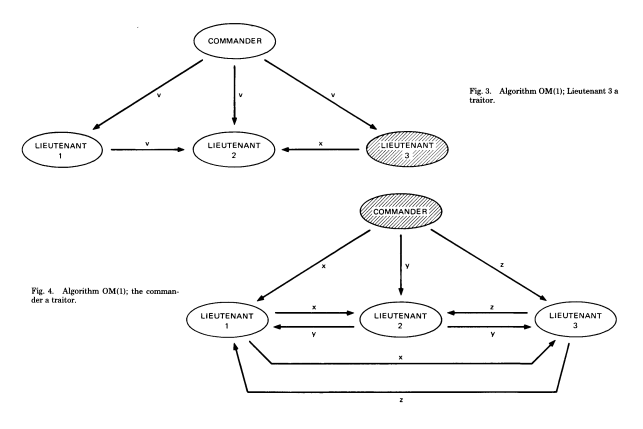
\includegraphics{commander_leutenants.png}
            \caption{Các trường hợp xảy ra trong bài toán chỉ huy và trung úy}
        \end{figure}
        \begin{itemize}
            \item Trường hợp 1, kẻ phản bội là L3. C sẽ gửi tin với nội dung v cho L1, L2, L3. L3 phản bội nên sẽ sửa đổi nội dung, và gửi x cho L2. Tuy nhiên, L2 sẽ nhận được v từ L1 và C và sẽ thấy là phần đông đã lựa chọn v. Từ đó những vị tướng trung thành, gồm C, L1 và L2 sẽ đạt được sự đồng thuận là phương án v, mặc cho L3 có gửi tin x.
            \item Trường hợp 2, kẻ phản bội là C. C có thể gửi x cho L1, gửi y cho L2 và gửi z cho L3. L1, L2, L3 đều trung thành, nên sẽ gửi tin mà họ nhận được cho những người khác. Như vậy L1 sẽ nhận được đủ cả 3 lệnh là x (từ C), y (từ L2) và z (từ L3). Trông có vẻ như không thể quyết định được đấy, nhưng thực chất, quyết định của cả 3 người sẽ là giống nhau, vì cùng là majority(x,y,z). Nếu x, y, z mang những nội dung hoàn toàn khác nhau, và không thể tính trọng số, tất cả sẽ theo lựa chọn default, ở đây có thể là rút quân chẳng hạn.
        \end{itemize}
    \end{enumerate}

    \subsection{Sinh viên Khoa Toán - Cơ - Tin học và con đường phát triển nghề nghiệp tại một tổ chức tài chính ngân hàng}
    
    Bài thuyết trình được thực hiện bởi ông Lê Công Bình, Trưởng Phòng Triển khai và Phát triển ứng dụng, Trung tâm CNTT ngân hàng BIDV.
    Ngân hàng BIDV là ngân hàng có vốn hóa lớn nhất Việt Nam.

    Các vị trí công việc trong phòng CNTT tại ngân hàng BIDV:

    \begin{itemize}
        \item Kế hoạch chiến lược:
        \begin{itemize}
            \item Kế hoạch chiến lược
            \item Quản lý dự án CNTT
            \item Quản lý kiến trúc tổng thể
            \item Nghiên cứu công nghệ mới
        \end{itemize}
        \item Phát triển ứng dụng
        \begin{itemize}
            \item Phân tích nghiệp vụ (BA)
            \item Lập trình viên (Frontend, Mid, Backend)
            \item Phân tích thiết Kế
            \item Tích hợp hệ thống
            \item Đảm bảo chất lượng QA - QC
        \end{itemize}
        \item Phân tích dữ liệu
        \begin{itemize}
            \item Báo cáo quản trị điều hành
            \item Data Governance
            \item Phân tích dữ liệu khách hàng
            \item Phân tích dữ liệu rủi ro
        \end{itemize}
        \item Quản trị hạ tầng
        \begin{itemize}
            \item Quản trị máy chủ, thiết bị lưu trữ
            \item Quản trị cơ sở dữ liệu
            \item Quản trị mạng, truyền thông
            \item Quản trị an ninh bảo mật
            \item Quản trị trung tâm dữ liệu
        \end{itemize}
    \end{itemize}

    Một số vị trí cho lập trình viên và các công nghệ hay được sử dụng tại các vị trí tương ứng:

    \begin{itemize}
        \item Chuyên viên phát triển phần mềm: ReactJS, AngularJS, SpringBoot, Sonarqube
        \item Chuyên viên tích hợp hệ thống
        \item Chuyên viên thiết kế hệ thống: IBM WebSphere, IBM Rational Software
        \item Chuyên viên cấp cao
        \item Chuyên gia
    \end{itemize}

    Các kỹ năng và kiến thức mà sinh viên cần chuẩn bị:

    \begin{itemize}
        \item Tinh thần học hỏi và liên tục phát triển bản thân
        \item Tự lập trình từ đầu đến cuối theo các chuẩn framework
        \item Kiến thức cơ bản cơ sở dữ liệu và thiết kế cơ sở dữ liệu
        \item Tìm hiểu một số xu thế công nghệ: Microservice, kiến trúc mở, cloud, Big Data
        \item Kỹ năng đọc hiểu tiếng Anh - Giao tiếp cơ bản. Mục tiêu TOEIC 600 điểm hoặc tương đương
        \item Kỹ năng mềm: Phối hợp làm việc nhóm, quản lý thời gian, xác lập mục tiêu cá nhân trong phát triển nghề nghiệp
    \end{itemize}
    %\section{Tham quan hội trại}

    \section{Chuỗi bài giản về khoa học dữ liệu}

    \subsection{Dự án giải mã 1000 hệ gen người Việt}

    Bài thuyết trình được thực hiện bởi TS. Võ Sỹ Nam, công ty GeneStory trình bày về dự án "Giải mã 1000 hệ gen người Việt".
    Bài thuyết trình đã đề cập đến lý thuyết cơ bản về DNA bao gồm: lịch sử ra đời mô hình, quá trình giải mã, các công trình nghiên cứu về nguồn gốc loài người dựa trên các công trình nghiên cứu về gen cũng như vai trò của việc giải mã gen trong kỷ nguyên của y học chính xác.

    Cấu trúc DNA được James Watson và Francis Crick đề xuất trong quá trình nghiên cứu tại Lab Cavendish năm 1953.
    Có nhiều thông tin cho rằng James Watson và Francis Crick đã lấy ý tưởng từ nhà nghiên cứu Rosalind Franklin tại Paris.
    DNA có cấu trúc xoắn kép. DNA chứa đựng các thông tin di truyền từ thế hệ này sang thế hệ khác nhờ khả năng phân đôi trong quá trình sinh sản và quyết định tất cả các đặc điểm của chúng ta. DNA có ở trong nhân tế vào và một lượng nhỏ nằm trong ty thể. 
    
    Thông tin trong DNA được lưu trữ dưới dạng mã, được tạo thành từ bốn loại bazơ nitơ là: adenine (A), guanine (G), cytosine (C) và thymine (T). Các bazơ này bắt cặp với nhau, A với T và C với G, thông qua các liên kết hydro để tạo thành các đơn vị được gọi là cặp bazơ.

    DNA có cấu trúc không gian dạng xoắn kép với 2 mạch song song. Thực tế, 2 mạch này xoắn đều xung quanh 1 mạch cố định và theo chiều ngược kim đồng hồ. Cấu trúc xoắn kép DNA của mỗi người là khác nhau, do đó mỗi chúng ta đều có các đặc điểm riêng biệt. Do có tính đặc thù nên nhờ phân tích DNA các nhà khoa học có thể khám phá ra sự phát triển và tiến hóa của mỗi giống loài cũng như tìm ra giải pháp tối ưu để hạn chế, điều trị các căn bệnh do đột biến DNA di truyền.

    Ngoài ra việc nghiên cứu DNA còn có thể giúp chúng ta tìm ra nguồn gốc loài người cũng như quá trình di cư của tổ tiên chúng ta.
    Công trình của các nhà khoa học tại Trung tâm nghiên cứu dữ liệu lớn tại Vingroup cho thấy di truyển người Việt có độ đa dạng cao

    \begin{figure}[h!]
        \centering
        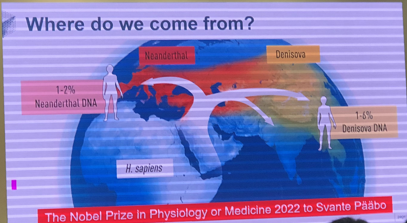
\includegraphics{immgrants_process.png}
        \caption{Quá trình di cư của loài người qua công trình nghiên cứu DNA}
    \end{figure}

    \begin{figure}[h!]
        \centering
        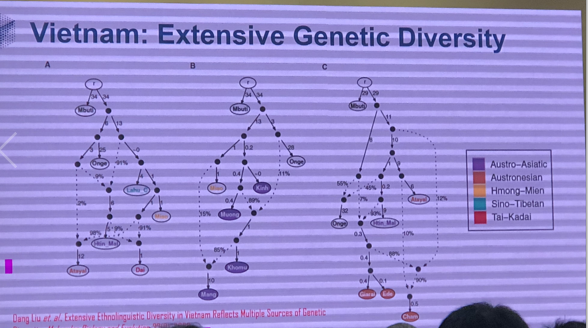
\includegraphics{Vietnam_Extensive_Genetic_Diversity.png}
        \caption{Độ đa dạng di truyền của người Việt}
    \end{figure}

    Với các tiến bộ về khoa học kỹ thuật, giải mã gen một người chỉ tốn khoảng 200 \$ và sẽ sớm đạt được 100 \$ (cách đây khoảng 20 năm chi phí này là hàng chục triệu \$)
    Ngoài ra việc giải mã gen người còn đặt ra những thách thức về công nghệ lưu trữ dữ liệu: Để giải mã gen 1008 người Việt cần dung lượng khoảng 1200 TB dữ liệu với 37 \% đến từ miền Bắc, 22 \% đến từ miền Trung, 41 \% đến từ miền Nam.
    
    \begin{figure}[h!]
        \centering
        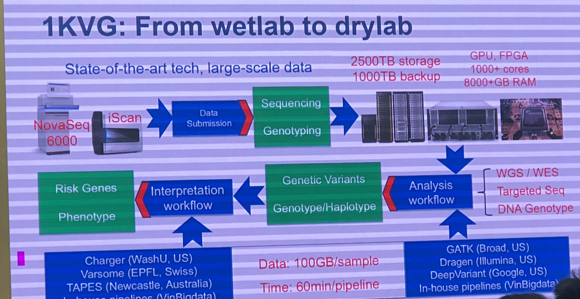
\includegraphics{Wetlab_to_Drylab.png}
        \caption{Quy trình giải mã gen từ máy giải trình tự đến các phân tích về gen}
    \end{figure}

    Để có thể làm việc với một lượng dữ liệu khổng lồ từ quá trình giải trình tự ta cần một nền tảng chuyên dụng cho dữ liệu lớn gồm các thành phần như: Apache Spark, Hadoop, Cassandra, Mesos, Apache HBase, Kubernetes, Elasticsearch.
    Các dữ liệu của công trình được chia làm hai phiên bản: Phiên bản 1 vào tháng 12/2020 với 58640 GB dữ liệu công khai và khoảng 450000 GB dữ liệu riêng tư. Phiên bản 2 vào tháng 12/2021 với 109308 GB dữ liệu mở và khoảng 1100000 GB dữ liệu riêng tư.

    Một vấn đề rất quan trọng nữa là làm thế nào để phân tích dữ liệu gen? Ban đầu ta cần thu thập được dữ liệu gen.
    Cả đoạn DNA của con người dài khoảng 3 tỷ ký tự. Nhưng ta chỉ có thể đọc được các đoạn phân mảnh khoảng 100 ký tự.
    Vậy câu hỏi đặt ra là làm sao ta có thể xây dựng lại cả DNA chỉ từ các phân mảnh ngắn? Một số phương pháp hay được dùng như là FASTQ, đọc gióng hàng trình tự DNA, hoặc sử dụng phương pháp Bayes để xác định các biến thể DNA và ánh xạ các phân mảnh nhỏ.

    Dữ liệu về gen của một người khoảng 50 - 70 GB dữ liệu và cần xử lý khoảng 500 - 700 GB dữ liệu qua toàn bộ quá trình xử lý.
    Để xử lý dữ liệu về gen của một người cần khoảng 30000 năm nếu sử dụng thuật toán Knuth-Morris-Pratt và khoảng 30 giờ nêu sử dụng thuật toán FM-Index.
    Ta giả sử một DNA có độ dài $n$ và độ dài từng phân mảnh đọc được là $m$ và $m \ll n$, $m \sim 10^2, n \sim 10^9$.
    Đối với vét cạn độ phức tạp là $O(mn)$, giả sử số lần đọc là $N=10^9$, mỗi phép tính cần $t=10^{-6}$(s) ta cần thời gian là $mnNt\sim$ 3 triệu năm.
    Đối với thuật toán Knuth-Morris-Pratt có độ phức tạp $O(m+n)$ ta cần thời gian là $(m+n)Nt\sim$ 30000 năm.

    Nhưng ta có thể khai thác và sử dụng gen như thế nào trong y tế? 
    Một ứng dụng nổi tiếng nhất của dữ liệu gen là y học chính xác, tùy thuộc vào kiểu gen mà sẽ có các cách điều trị ứng với từng bệnh.
    Ứng dụng khác là dự đoán các bệnh có thể gặp phải bằng việc phân tích và phát hiện các đoạn gen nguy cơ cao gây một loại bệnh nào đó.
    Một vài ứng dụng khác có thể kể đến như phát hiện phản ứng có hại với thuốc dựa trên dữ liệu gen, khả năng kháng thuốc của các loại vi khuẩn, vi-rút 


    \begin{figure}[h!]
        \centering
        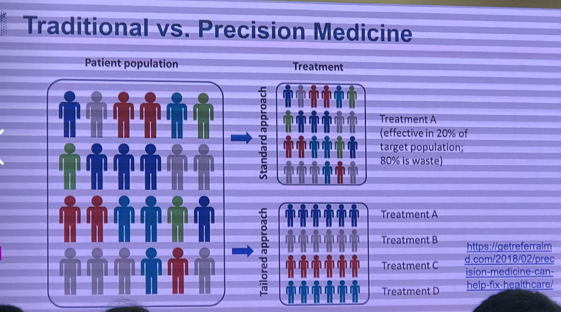
\includegraphics{Precise_Medicine.png}
        \caption{So sánh y học truyền thống và y học chính xác}
    \end{figure}

    \begin{figure}[h!]
        \centering
        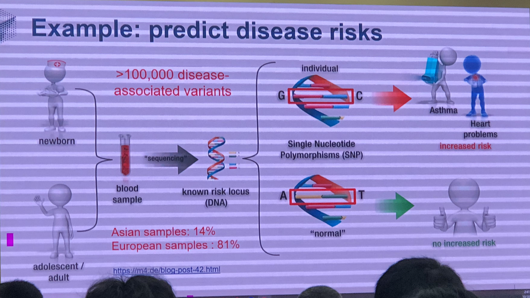
\includegraphics{predict-disease-risk.png}
        \caption{Dự đoán nguy cơ mắc các bệnh dựa trên dữ liệu gen}
    \end{figure}

    \subsection{Ứng dụng KHDL hỗ trợ khách hàng ra quyết định đầu tư thông minh tại TCBS (Techcom Securities)}

    Bài thuyết trình được thực hiện bởi ông Phạm Xuân Dũng, Senior Manager, Data Scientist, Bộ phận Phân tích, nâng cao và sáng tạo (AnI) Công ty TCBS, Techcombank về chủ đề "Ứng dụng KHDL hỗ trợ khách hàng ra quyết định đầu tư thông minh tại TCBS (Techcom Securities)"
    Diễn giả đã trình bày một số bài toán về tối ưu hóa danh mục đầu tư, phát hiện khách hàng tiềm năng từ dữ liệu hoạt động, phát hiện các mẫu hành động và dự đoán hành động tiếp theo của khách hàng.

    Các phương pháp tối ưu hóa danh mục đầu tư giúp khách hàng tiếp cận dữ liệu và mô hình tài chính để tự ra quyết định.

    \begin{figure}
        \centering
        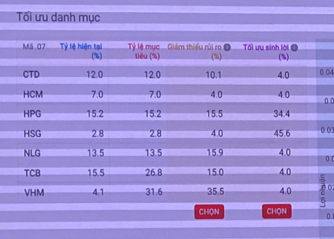
\includegraphics{Portfolio_Optimization.png}
        \caption{Ví dụ tối ưu hóa danh mục đầu tư từ một tập mã chứng khoán}
    \end{figure}

    Một số phương pháp để tối ưu hóa danh mục đầu tư: mô hình mean-variance, mô hình boosting,...
    Ngoài ra còn một số mô hình gợi ý các mã cổ phiếu dựa trên dữ liệu hoạt động của khách hàng.

    
    \begin{figure}[h!]
        \centering
        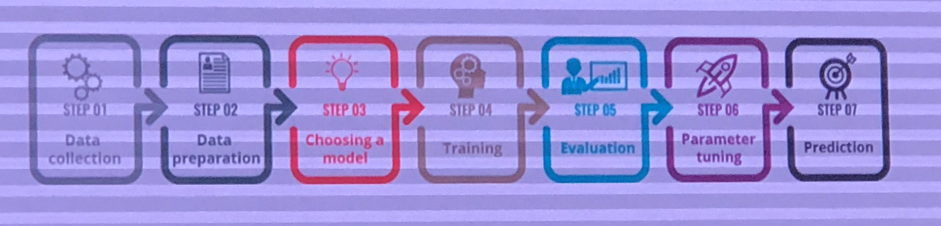
\includegraphics[scale=0.6]{TCBS_ML_Workflow.png}
        \caption{Machine Learning Workflow được thực hiện tại TCBS}
    \end{figure}

    \subsection{Data Analytics: Leading continuous improvement and predicting trends}

    Bài thuyết trình được thực hiện bởi ong David Lapetina, Giám đốc điều hành Công ty TIBCO Orchestra Networks Vietnam về chủ đề "Data Analytics: Leading continuous improvement and predicting trends".
    Bài thuyết trình đã đề cập một số vấn đề về:

    \begin{itemize}
        \item Data Analytics và Visual Analytics
        \item Khoa học dữ liệu
        \item Kinh doanh thông minh
        \item Hyperconverged Analytics
    \end{itemize}

    Ngoài ra một sản phẩm của TIBCO được giới thiệu là Spotfire.
    Spotfire là một nền tảng phân tích cấp doanh nghiệp cực kỳ mạnh mẽ dùng để thu thập những hiểu biết kinh doanh có giá trị. Đây là một công cụ thông minh, an toàn, linh hoạt và có thể mở rộng cung cấp khả năng trực quan hóa, khám phá, xử lý dữ liệu và phân tích dự đoán. Spotfire cũng bao gồm một bảng điều khiển (dashboard) hiệu quả và các ứng dụng phân tích tương tác.

    Spotfire cho phép người dùng kết hợp dữ liệu trong một phân tích duy nhất và có được một cái nhìn tổng thể về cùng một hình ảnh trực quan tương tác. Phần mềm Spotfire làm cho các doanh nghiệp trở nên thông minh, cung cấp phân tích dựa trên AI và giúp việc vẽ dữ liệu tương tác trên bản đồ trở nên dễ dàng hơn.

    Nền tảng này giúp các doanh nghiệp chuyển đổi dữ liệu của họ thành những thông tin chi tiết mạnh mẽ một cách dễ dàng và tốn ít thời gian hơn. Nó tăng tốc độ phân tích dữ liệu trong một tổ chức để đưa ra quyết định nhanh hơn, tự tin và chính xác hơn nhiều.

    Các công ty hiện đang tràn ngập lượng dữ liệu có cấu trúc và phi cấu trúc khổng lồ từ các nguồn khác nhau và việc phân tích dữ liệu là khá khó khăn. Tuy nhiên, các kỹ thuật khám phá dữ liệu ngày nay được hỗ trợ bởi AI và Machine Learning đưa việc phân tích dữ liệu lên một tầm cao mới. Spotfire cho phép khám phá dữ liệu, nơi chúng ta có thể tìm kiếm dữ liệu giống như tìm kiếm trên web đơn giản.

    Trực quan hóa dữ liệu (Data Visualization) là một biểu diễn đồ họa của dữ liệu. Spotfire trực quan hóa, tương tác và chia sẻ dữ liệu để tìm ra rủi ro và cơ hội trong phân tích. Spotfire triển khai trực quan hóa thông qua đồ thị, biểu đồ 3D và các dạng tương tác khác.

    Phân tích dự đoán bao gồm các kỹ thuật thống kê nhất định như Học máy, khai thác dữ liệu và mô hình dự đoán để phân tích dữ liệu hiện tại và lịch sử, đồng thời dự đoán các diễn biến trong tương lai hoặc các sự kiện chưa biết.

    Trong phân tích dự đoán dùng Spotfire, chúng ta có thể dự đoán các xu hướng mới nổi, thực hiện các hành động phủ đầu để giảm thiểu rủi ro và đưa ra quyết định tốt hơn với sự tự tin cao hơn nhiều.
    \subsection{Ứng dụng của toán học hiện đại và khoa học dữ liệu để giải quyết các bài toán trong lĩnh vực chuỗi cung ứng}

    Bài thuyết trình được thực hiện bởi ông Đỗ Huy Bình - Tổng Giám Đốc và TS. Đỗ Đức Hạnh - Trưởng phòng nghiên cứu toán học và AI, 
    Smartlog về chủ đề "Ứng dụng của toán học hiện đại và khoa học dữ liệu để giải quyết các bài toán trong lĩnh vực chuỗi cung ứng"
    
    Smartlog đang xây dựng một hệ sinh thái tích hợp Logistics tốt nhất tại Việt Nam cũng như Đông Nam Á.
    Mục tiêu đến năm 2025 chiếm 10 \% thị phần thị trường Logistics.
    Tầm nhìn trở thành nền tảng và hệ sinh thái tích hợp đầu tiên cho hoạt động logistics với phạm vi bao phủ lớn nhất tại Việt Nam - Đông Nam Á.
    Sứ mệnh tham gia cung cấp và cải tiến hiệu suất cho tất cả các bên liên quan trong chuỗi cung ứng thông qua nền tảng toàn diện bằng cách đẩy mạnh công nghệ, con người và tài sản.

    \begin{figure}[h!]
        \centering
        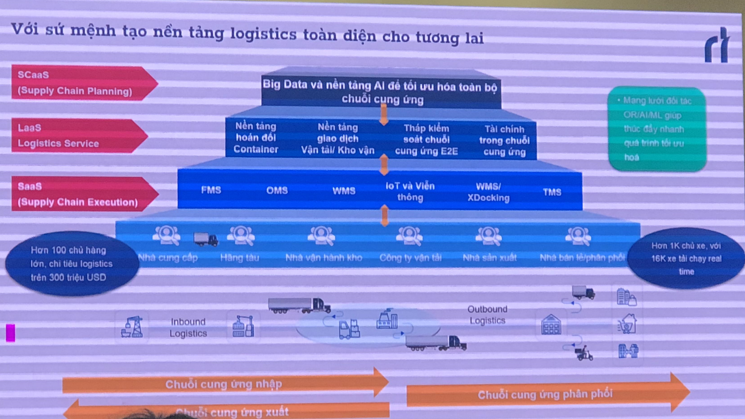
\includegraphics[scale=0.6]{Smartlog_Infra.png}
        \caption{Nền tảng kiến trúc Logistics của Smartlog}
    \end{figure}

    Smartlog đồng hành cùng rất nhiều khách hàng là những nhà sản xuất và phân phối đầu ngành như: Sabeco - công ty dẫn đầu ngành đồ uống, Abbott - sản xuất và phân phối sữa, OneMount - công ty dẫn đầu về phân phối FMCG, Brenntag - sản xuất và phân phối các sản phẩm hóa chất cho nhiều ngành, Saint - Gobain - sản xuất và phân phối các sản phẩm xây dựng.

    Dấu chân của Smartlog đã đặt trên mọi miền đất nước với hệ thống kho vận SWM xử lý gần 4 triệu đơn hàng, hơn 50 nghìn SKU quản lý, hơn 100 kho hàng và hơn 3000 Hub.
    Hệ thống vận tải STM với hơn 20 nghìn xe chạy trên toàn hệ thống, hơn 67 nghìn chuyến/tháng được điều phối và giám sát trên STM, hơn 100 khách hàng đang sử dụng TMS.
    Và đa dạng loại hình vận chuyển như Containers, Inbound Logistics, phân phối và last mile (xe máy).

    \begin{figure}[h!]
        \centering
        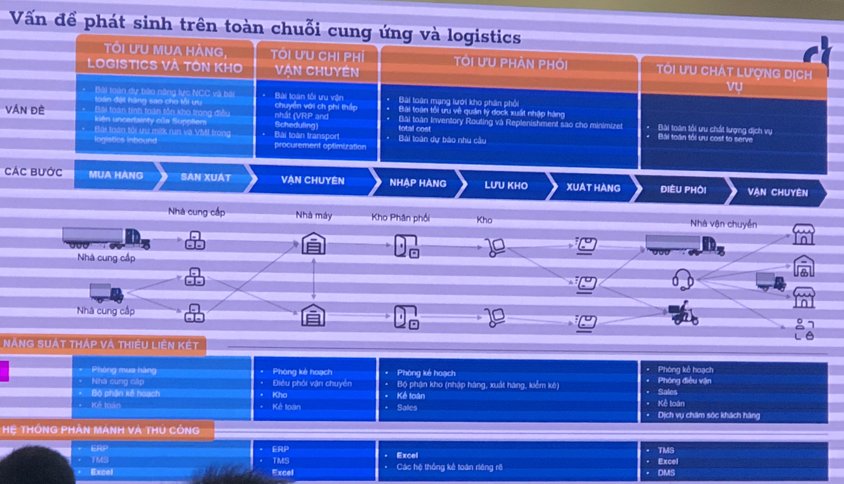
\includegraphics[scale=0.6]{Logistic_Problem.png}
        \caption{Các vấn đề phát sinh trên toàn chuỗi cung ứng và Logistics}
    \end{figure}

    Các xu hướng impact rất lớn trong ngành SC và Logistics:

    \begin{itemize}
        \item Sự phát triển của thương mại điện tử và đa kênh: chất lượng dịch vụ cộng với sự gia tăng nhóm khách hàng B2C, mạng lưới giao hàng phức tạp, mạng lưới tồn kho rộng lớn.
        \item Chuỗi cung ứng và Logistics: chuỗi cung ứng ngày càng quan trọng và phức tạp, Logistics đang là lợi thế cạnh tranh, chi phí Logistics rất ca và vận hành kém hiệu quả.
        \item Kinh tế chia sẻ và công nghệ đang lên ngôi: sự phát triển của SaaS và LaaS đang làm cho mọi thứ trở nên dễ dàng hơn, dữ liệu nhiều hơn và tiềm năng hơn, sự cộng tác mở rộng ngày càng lớn hơn.
    \end{itemize}

    Một số bài toán mà Smartlog đang cần giải với khách hàng của mình:

    \begin{itemize}
        \item Tối ưu hóa vận chuyển containter với các ràng buộc đặc thù
        \item Bài toán routing với nhiều mô hình kết hợp (kết hợp xe tải, xe máy, kết hợp cross docking)
        \item Phân cụm
        \item Dự đoán lượng tồn kho tối ưu
        \item Bài toán sắp xếp hàng trong kho sao cho tối ưu trên cơ sở phân tích dữ liệu hành vi mua hàng
        \item Bài toán tối ưu inventory routing để giao hàng
        \item Bài toán matching giữa người mua và bán dịch vụ sao cho tối ưu chi phí và dịch vụ
    \end{itemize}

    \section{Bài toán tối ưu hóa định tuyến vận tải đa phương tiện sử dụng các thuật toán xấp xỉ}

    Mục tiêu của bài toán là tạo ra một tuyến đường tối ưu cho bài toán định tuyến vận tải nhiều phương tiện (mVRP).
    Ta sử dụng phương pháp phân cụm các thành phố biết trước dựa trên số phương tiện và từng cụm sẽ được phân bổ vào một phương tiện.
    Thuật toán k-Means được sử dụng cho việc phân cụm các thành phố.
    Sau khi phân cụm hoàn tất, một tuyến đường tối ưu được tạo ra cho từng phương tiện.
    Khi các thành phố được gán cho các phương tiện, từng cụm sẽ được coi như là một bài toán định tuyến vận tải và sử dụng thuật toán di truyền để tìm giá trị tối ưu khoảng cách sau khi hội tụ.
    Giải thuật di truyền trong trường hợp này tốt hơn các kỹ thuật heuristics và có chi phí tính toán thấp hơn.

    Một vài survey đã tóm tắt các biến thể và các phương pháp của bài toán tối ưu hóa tổ hợp cho thấy một số biến thể có thể giải được bằng các kỹ thuật metaheuristics ví dụ:

    \begin{itemize}
        \item Bài toán định tuyến vận tải đa phương tiện (mVRP)
        \item mVRP với phân bổ cân bằng giữa các nút với hàm mục tiêu đơn hoặc đa hàm mục tiêu
    \end{itemize}

    Trong bài toán định tuyến vận tải, số thành phố cần phải đi qua bởi một phương tiện cần được trả về cùng một thành phố nơi mà phương tiện này xuất phát.
    Khi giải bài toán ta cần thử xây dựng tuyến đường mà tổng khoảng cách đi là nhỏ nhất.
    Tất cả các phương tiện bắt đầu từ cùng thành phố gọi là kho và phải quay về đúng nơi này là điểm kết thúc của hành trình.

    Nếu $n$ là số thành phố cần qua thì có $(n-1)!$ số tuyến đường khả dĩ.
    Vì vậy thay vì xem xét tất cả các tuyến đường khả dĩ, các kỹ thuật heuristic giải bài toán định tuyến vận tải có khả năng giảm đáng kể số tuyến đường khả dĩ cần được xem xét.

    Tổng quát hóa của bài toán tối ưu định tuyến vận tải là bài toán tối ưu hóa định tuyến vận tải đa phương tiện (mVRP), bao gồm xác định một tập tuyến đường cho $m$ phương tiện.
    mVRP có thể được định nghĩa như sau: Cho một tập các nút, $m$ phương tiện được đặt tại một nhà khi tại một nút nào đó. Các nút còn lại (thành phố) cần được đi qua gọi là các nút trung gian.
    Bài toán mVRP là tìm những tuyến đường cho tất cả $m$ phương tiện mà điểm xuất phát và điểm bắt đầu là một, và các điểm nút trung gian được đi qua đúng một lần và tổng chi phí đi qua các nút là nhỏ nhất.

    Cấu trúc toán học của bài toán định tuyến vận tải là một đồ thị mà các thành phố là các nút của đồ thị.
    Các kết nối giữa các cặp thành phố gọi là cạnh và từng cạnh có một chi phí tương ứng có thể là khoảng cách, thời gian hoặc một thuộc tính khác.
    Nếu $n$ là số đỉnh biểu diễn các thành phố, cho một đồ thị có hướng $G$,
    bài toán định tuyến vận tải là tìm một chu trình với chi phí nhỏ nhất đi qua từng đỉnh của $G$ đúng một lần.

    Có nhiều cách biểu diễn hình thức toán học của bài toán định tuyến vận tải VRP, và có nhiều kiểu ràng buộc của bài toán.
    Các ký hiệu chính thức:
    \begin{itemize}
        \item $n$ là số thành phố cần được đi qua, số đỉnh có trong đồ thị
        \item $i, j, k$ chỉ số của các thành phố được đánh số từ $1$ đến $n$
        \item $t$ là chỉ số bước thời gian
        \item $x_{ijt}$ có giá trị là 1 nếu cạnh của đồ thị từ đỉnh $i$ đến đỉnh $j$ và đi ở bước $t$ trong định tuyến.
        \item $d_{ij}$ là khoảng cách hoặc chi phí từ đỉnh $i$ đến đỉnh $j$
    \end{itemize}

    Ví dụ về một bài toán định tuyến vận tải quy hoạch tuyến tính:

    \begin{itemize}
        \item Hàm mục tiêu $Z$ cần được cực tiểu hóa là tổng của tổng chi phí của tất cả các phần tử trong định tuyến:
        \begin{equation}
            Z = \sum_{i=1}^n \sum_{j=1}^n \sum_{t=1}^n d_{ij} x_{ijt}
        \end{equation}
        \item Ràng buộc với tất cả các giá trị thời gian $t$ chỉ có một cung đường được chọn:
        \begin{equation}
            \sum_{i=1}^n \sum_{j=1}^n x_{ijt} = 1 \forall t
        \end{equation}
        \item Với từng thành phố chỉ có duy nhất một thành phố khác có xe đi đến tại mỗi một thời điểm:
        \begin{equation}
            \sum_{j=1}^n \sum_{t=1}^n x_{i j t}=1 \forall i
        \end{equation}
        \item Với từng thành phố chỉ có duy nhất một thành phố khác mà nó đi đến tại mỗi một thời điểm:
        \begin{equation}
            \sum_{i=1}^n \sum_{t=1}^n x_{ijt}=1 \forall i
        \end{equation}
        \item Khi một thành phố có một xe đến tại thời điểm $t$, xe này cần được rời ở thời điểm $t+1$:
        \begin{equation}
            \sum_{i=1}^n x_{i j t} = \sum_{k=1}^n x_{j k t + 1} \forall j \forall t
        \end{equation}
        \item Ngoài ra các biến quyết định $x_{i j t}$ chỉ có thể nhận giá trị 0 hoặc 1:
        \begin{equation}
            0 \leq x_{i j t} \leq 1
        \end{equation}
    \end{itemize}

    Ta giả định các phương tiện xuất phát từ nhà kho đi qua một tập các thành phố và phải quay về đúng điểm xuất phát.
    Không có ràng buộc về chi phí nhưng mỗi thành phố chỉ được các phương tiện đi qua đúng một lần.

    Không gian tìm kiếm cho lời giải tắc lên khi số thành phố tăng lên.
    Nếu có $N$ thành phố thì không gian tìm kiếm có lực lượng là $N!$ và chi phí tính toán sẽ rất cao.
    Để giảm gánh nặng chi phí tính toán thì số thành phố cần được giảm bằng phân cụm.

    k-means là một thuật toán phân loại hoặc phân nhóm các vật thể vào $k$ nhóm, $k$ là một số nguyên dương.
    Quá trình gom nhóm được thực hiện bằng cách cực tiểu hóa tổng các bình phương khoảng cách giữa dữ liệu và trọng tâm của cụm tương ứng.

    Ý tưởng chính là để xác định $k$ trọng tâm cho từng cụm. Từng trọng tâm cần được chọn hợp lý vì với các cách chọn trọng tâm khác nhau sẽ dẫn đến kết quả khác nhau.
    Một cách chọn tốt là chọn các trọng tâm ban đầu càng xa các trọng tâm còn lại càng tốt.
    Bước tiếp theo là chọn từng điểm thuộc về cụm nào bằng cách gán vào cụm ứng với trọng tâm gần nhất.
    
    Khi không còn điểm nào để gán, bước đầu tiên đã hoàn thành.
    Ta cần tính lại vị trí của $k$ trọng tâm mới của từng cụm từ bước trước.
    Sau khi đã tính $k$ trọng tâm mới, một bước tiếp theo là lại gán các điểm dữ liệu và cụm có trọng tâm tương ứng gần với nó nhất.
    Một bước lặp lại được thực hiện. Ta sẽ dừng lại khi mà vị trí $k$ điểm trọng tâm không thay đổi nhiều.

    Thủ tục của thuật toán k-means là:

    \begin{algorithm}[h!]
        \DontPrintSemicolon
        \KwIn{Các điểm dữ liệu $x^{(1)}, x^{(2)}, \dots, x^{(n)}, k$}
        \KwOut{$k$ điểm trọng tâm của từng cụm}
        Khởi tạo các điểm trong tâm $\mu_1, \mu_2, \dots, \mu_k$ một cách ngẫu nghiên\;
        \Repeat{hội tụ} {
            \For{$i \gets 1$ \textbf{to} $n$} {
                $c^{(i)} \gets \underset{j}{\mathrm{argmin}} \lVert x^{(i)} - \mu_j \rVert_2^2$\;
            }
            \For{$i \gets 1$ \textbf{to} $k$} {
                $\mu_j \gets \dfrac{\sum_{i=1}^n 1\lbrace c^{(i)} = j \rbrace x^{(i)}}{\sum_{i=1}^n 1\lbrace c^{(i)} = j \rbrace}$\;
            }
        }
        \Return{$\mu_1, \mu_2, \dots, \mu_k$}\;
    \end{algorithm}

    Tiếp đến ta sẽ áp dụng giải thuật di truyền vào bài toán tối ưu hóa định tuyến đa phương tiện (mVRP).
    Giải thuật di truyền giả lập cơ chế chọn lọc tự nhiên.
    Giải thuật di truyền tạo ra một quần thể các vector số học gọi là nhiễm sắc thể,
    mỗi nhiễm sắc thể biểu diễn một lời giải có thể của bài toán.
    Các thành phần độc lập trong nhiễm sắc thể được gọi là gen.
    Những nhiễm sắc thể mới được tạo bởi lai hoặc đột biến.
    Sau đó những nhiễm sắc thể được đánh giá dựa trên hàm phù hợp.
    Những nhiễm sắc thể càng phù hợp xác suất sống sót càng cao hơn.
    Quần thể gen tiến hóa theo từng thế hệ và tạo ra những lời giải ngày càng tốt hơn.
    Quá trình thực hiện giải thuật di truyền sẽ dừng khi giá trị hàm phù hợp đạt đến một giá trị đặt trước,
    hoặc sau một khoảng thời gian đủ dài hoặc khi mà không có sự cải thiện nhiều ở giá trị hàm phù hợp trong một số bước lặp liên tiếp.
    Mấu chốt của lời giải sử dụng giải thuật di truyền nằm ở việc sử dụng một biểu diễn nhiễm sắc thể của các lời giải bài toán một cách phù hợp.

    Mã giả giải thuật di truyền:

    
    \newpage
    \addcontentsline{toc}{section}{TÀI LIỆU THAM KHẢO}
    \printbibliography[title={TÀI LIỆU THAM KHẢO}]

\end{document}